\graphicspath{{./fig_Rayleigh/}}

\subsection{Rayleigh流れ}

%
\subsubsection{目的}
粘性の時間的な影響を厳密解と比較し,粘性項の計算精度を調べる.

%
\subsubsection{問題の定義と厳密解}

無限平板の平板面内の非定常運動によって生じる流れの問題で,\textbf{図\ref{}}のように平板が面内で突然一定方向に一定速度$U_0$で動き出す場合である\cite{hino:74:fd}.
レイノルズ数は層流域内で,完全な二次元平行流で圧力勾配と外力はないと仮定する.この場合,Navier-Stokes方程式は\textbf{式(\ref{eq:Stokes 1 eq})}のようになる.

\begin{equation}
\frac{\partial u}{\partial t}
\,=\,
\nu \frac{\partial^2 u}{\partial y^2}
\label{eq:Stokes 1 eq}
\end{equation}

\vspace{3mm}
初期条件と境界条件は,次のようになる.

\begin{equation}
\left .
\begin{array}{llll}
\vspace{2mm}
t \le 0 & ; & u=0 & ( \forall y )\\
t > 0 & ; & u=U_0 & (y=0)\\
& ; & u \rightarrow 0 & (y \rightarrow \infty)\\
\end{array} \quad \right \}
\label{eq:Stokes 1 init}
\end{equation}

代表長さとして境界層厚さ$\delta$,代表速度を$U_0$にとると,\textbf{式(\ref{eq:Stokes 1 eq})}のオーダーは$U_0 \slash T \,\sim \, \nu U_0 \slash \delta^2$から$\delta \sim \sqrt{\nu t}$である.$y=2\sqrt{\nu t}\,\eta$と変数変換し,
解の形として$u(y,t)=U_0\,f(\eta)$を仮定すると,\textbf{式(\ref{eq:Stokes 1 eq})}と\textbf{式(\ref{eq:Stokes 1 init})}は,次式のように変換される.

\begin{equation}
\left.
\begin{array}{l}
\vspace{2mm}
f^{\prime \prime} + 2 \eta f^{\prime}=0 \\
\qquad f=1\quad(\eta=0)\\
\qquad f \rightarrow 0\,\,\,\,(\eta \rightarrow \infty)\\
\end{array}
\quad \right\}
\label{eq:Stokes 1 : trans}
\end{equation}

$f^{\prime}=F$とおくと,上式は$F^{\prime}+2\eta F=0$の線形常微分方程式で,$u$は次の形式となる.

\begin{equation}
\frac{u}{U_0} \,=\, (1-\mathrm{erf}\, \eta)
\label{eq:Stokes 1 : solution}
\end{equation}

\noindent ここで$\mathrm{erf}(\eta)$は誤差関数を表し,

\begin{equation}
\mathrm{erf}\, \eta \,=\, \frac{2}{\sqrt{\pi}} \int_0^{\,\eta} {e^{-\xi^2}}d\xi
\label{eq:error function}
\end{equation}

\noindent である.$y\slash U_0 \sim \eta$で整理された無次元のプロファイルは\textbf{図\ref{fig:Rayleigh profile}}のようになる.

\begin{figure}[htdp]
\begin{center}
\includegraphics[width=5cm,clip]{exact.eps}
\end{center}
\caption{相似流速分布\cite{hino:74:fd}}
\label{fig:Rayleigh profile}
\end{figure}

流束分布は相似形となる.境界層厚さ$\delta$を流速が壁面速度の約0.5\%になる距離で定義すると,$\mathrm{erf}(\eta)=0.9953$のとき$\eta=2$となる.

\begin{equation}
\delta(t) \,=\, 4 \sqrt{\nu t}
\label{eq:Stokes 1 : boundary layer}
\end{equation}

つまり,粘性の影響は動粘性係数と時間の平方根に比例して遠方に広がる.

%
\subsubsection{計算問題の準備}
作動流体として空気($\nu=1.5\times 10^{-5}\,[m^2/s]$)を考えると,\textbf{式(\ref{eq:Stokes 1 : boundary layer})}から10秒後の粘性の及ぶ範囲は$\delta \sim 4.7\times 10^{-2}\,[m]$,つまり5cm程度となる.


%
\subsubsection{計算環境}


%
\subsubsection{計算結果と厳密解の比較}


%
\subsubsection{参考文献}



